\documentclass[journal,12pt,twocolumn]{IEEEtran}

\usepackage{enumitem}
\usepackage{amsmath}
\usepackage{amssymb}
\usepackage{gensymb}
\usepackage{graphicx}
\usepackage{txfonts}         
\usepackage{listings}
\usepackage{lstautogobble}
\usepackage{mathtools}
\usepackage{bm}
\usepackage{hyperref}
\usepackage{polynom}
\usepackage{capt-of}
\newcommand{\solution}{\noindent \textbf{Solution: }}
\providecommand{\pr}[1]{\ensuremath{\Pr\left(#1\right)}}
\providecommand{\brak}[1]{\ensuremath{\left(#1\right)}}
\providecommand{\cbrak}[1]{\ensuremath{\left\{#1\right\}}}
\providecommand{\sbrak}[1]{\ensuremath{\left[#1\right]}}
\providecommand{\mean}[1]{E\left[ #1 \right]}
\providecommand{\var}[1]{\mathrm{Var}\left[ #1 \right]}
\providecommand{\der}[1]{\mathrm{d} #1}
\providecommand{\gauss}[2]{\mathcal{N}\ensuremath{\left(#1,#2\right)}}
\providecommand{\mbf}{\mathbf}
\providecommand{\abs}[1]{\left\vert#1\right\vert}
\providecommand{\norm}[1]{\left\lVert#1\right\rVert}
\providecommand{\z}[1]{{\mathcal{Z}}\{#1\}}
\providecommand{\ztrans}{\overset{\mathcal{Z}}{ \rightleftharpoons}}

\providecommand{\parder}[2]{\frac{\partial}{\partial #2} \brak{#1}}

\let\StandardTheFigure\thefigure
\let\vec\mathbf

\numberwithin{equation}{section}
\renewcommand{\thefigure}{\theenumi}
\renewcommand\thesection{\arabic{section}}

\newcommand{\myvec}[1]{\ensuremath{\begin{pmatrix}#1\end{pmatrix}}}
\newcommand{\mydet}[1]{\ensuremath{\begin{vmatrix}#1\end{vmatrix}}}
\newcommand{\define}{\stackrel{\triangle}{=}}

\DeclareMathOperator*{\argmin}{arg\,min}
\DeclareMathOperator*{\argmax}{arg\,max}


\lstset {
	frame=single, 
	breaklines=true,
	columns=fullflexible,
	autogobble=true
}             
   


\begin{document}
                             
\title{ Digital Signal Processing \\ \Large EE3900: Linear Systems and Signal Processing \\ \large Indian Institute of Technology Hyderabad \\ \vspace*{12pt} \textbf{Pingala}}
\author{Lokesh Badisa \\ \normalsize AI21BTECH11005 \\ \vspace*{20pt} \normalsize 7 Oct 2022  }
 \maketitle 
 \tableofcontents 
\section{JEE 2019}
\noindent Let $\alpha$ and $\beta$ ($\alpha > \beta$) be the roots of the
equation $z^2 - z - 1 = 0$. Define,
\begin{align}
	a_n &= \frac{\alpha^{n}-\beta^{n}}{\alpha - \beta}, \quad n \ge 1
	\\
	b_n &= a_{n-1} + a_{n+1}, \quad n \ge 2, \quad b_1 =1
	\label{eq:10-orig-diff}
\end{align}
Verify the following using a python code.
\begin{enumerate}[label=\thesection.\arabic*
,ref=\thesection.\theenumi]
\item 
\begin{align}
	\sum_{k=1}^{n}a_k = a_{n+2}-1, \quad n \ge 1
\end{align}
\solution
\begin{lstlisting}
https://raw.githubusercontent.com/LokeshBadisa/EE3900-Linear-Systems-and-Signal-Processing/main/pingala/codes/1.1.py
\end{lstlisting}
\begin{figure}[!ht]
    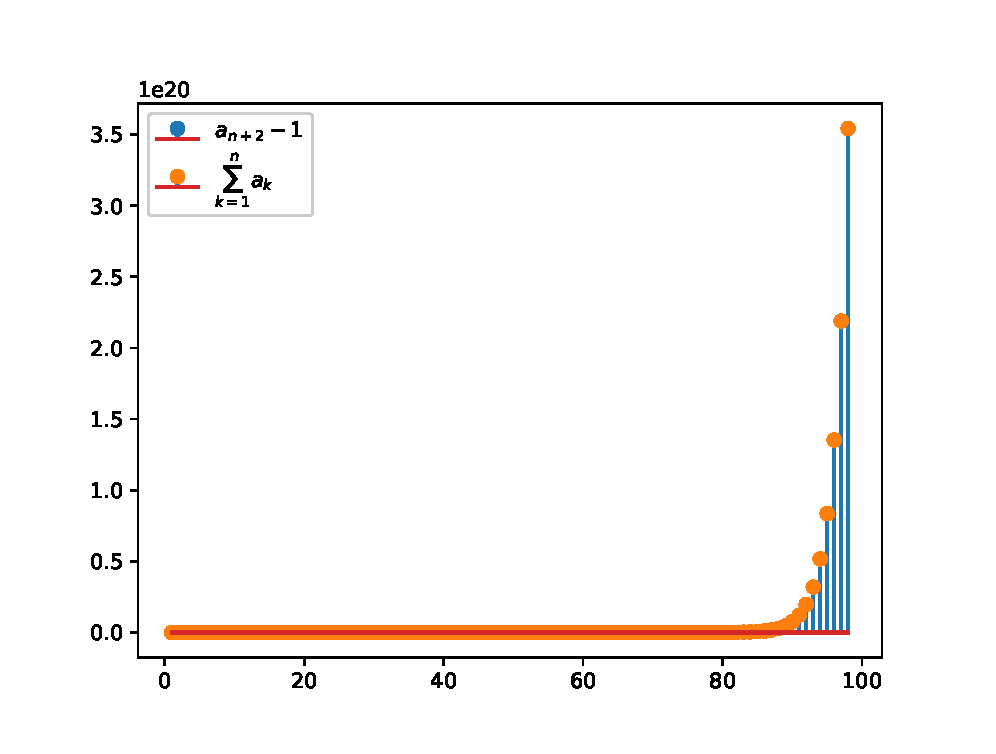
\includegraphics[width=\columnwidth]{figs/1.1}
\end{figure}
 \item 
\begin{align}
	\sum_{k=1}^{\infty}\frac{a_k}{10^k} =\frac{10}{89}
\end{align}
\solution
\begin{lstlisting}
https://raw.githubusercontent.com/LokeshBadisa/EE3900-Linear-Systems-and-Signal-Processing/main/pingala/codes/1.2.py
\end{lstlisting}
\begin{figure}[!ht]
    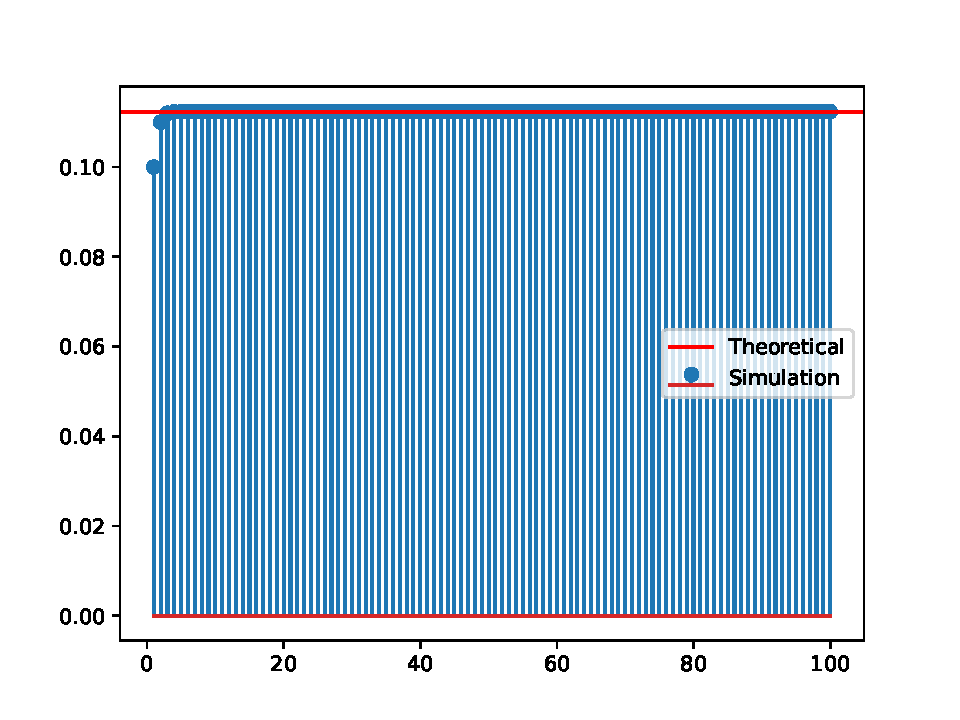
\includegraphics[width=\columnwidth]{figs/1.2}
\end{figure}
 \item 
\begin{align}
	b_n =\alpha^n + \beta^n, \quad n \ge 1
\end{align}
\solution
\begin{lstlisting}
https://raw.githubusercontent.com/LokeshBadisa/EE3900-Linear-Systems-and-Signal-Processing/main/pingala/codes/1.3.py
\end{lstlisting}
\begin{figure}[!ht]
    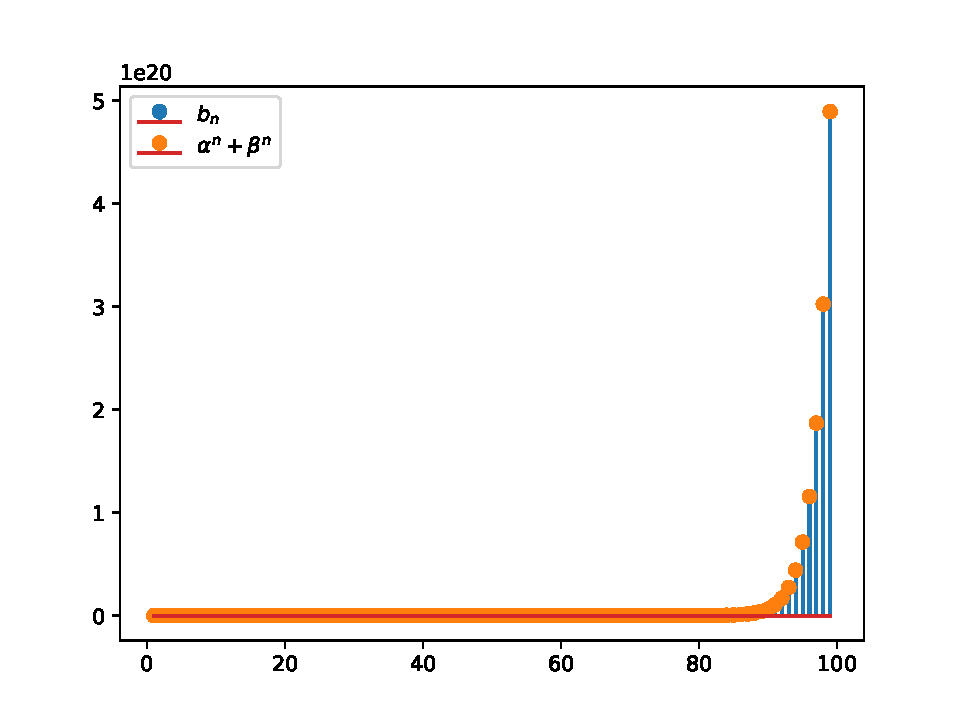
\includegraphics[width=\columnwidth]{figs/1.3}
\end{figure}
 \item 
\begin{align}
	\sum_{k=1}^{\infty}\frac{b_k}{10^k} =\frac{8}{89}
\end{align}
\solution
\begin{lstlisting}
https://raw.githubusercontent.com/LokeshBadisa/EE3900-Linear-Systems-and-Signal-Processing/main/pingala/codes/1.4.py
\end{lstlisting}
\begin{figure}[!ht]
    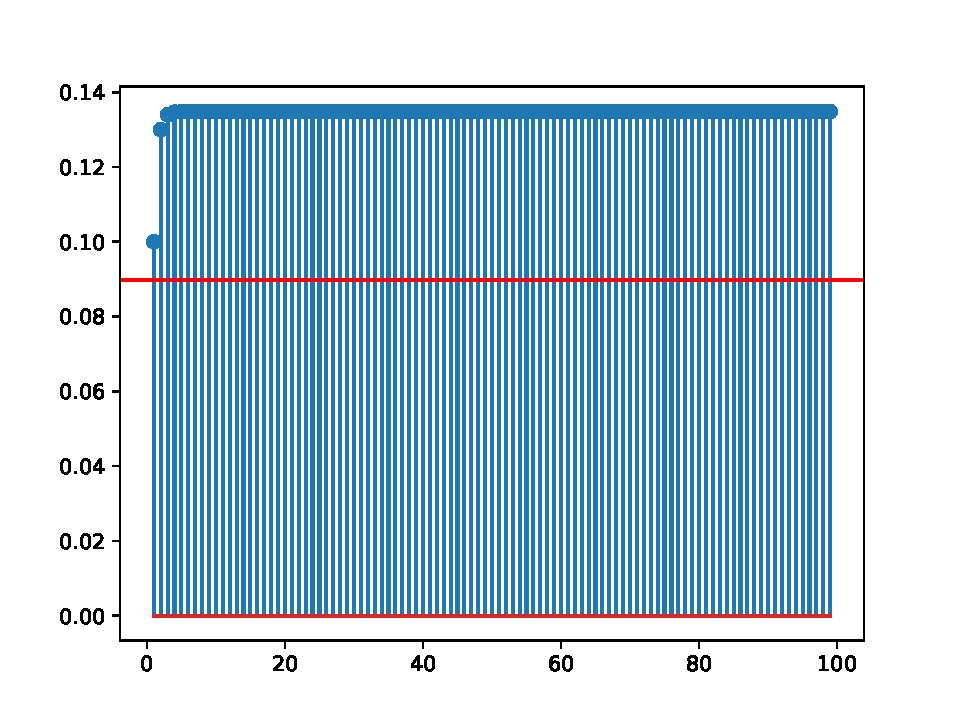
\includegraphics[width=\columnwidth]{figs/1.4}
\end{figure}
\end{enumerate}
\section{Pingala Series}
\begin{enumerate}[label=\thesection.\arabic*,ref=\thesection.\theenumi]
\item The {\em one sided} $Z$-transform of $x(n)$ is defined as 
\begin{align}
	X^{+}(z) = \sum_{n = 0}^{\infty}x(n)z^{-n}, \quad z \in \mathbb{C}
\label{eq:one-Z}
\end{align}
	\item The {\em Pingala} series is generated using the difference equation 
\begin{align}
	x(n+2) = x\brak{n+1} + x\brak{n},  \quad x(0) = x(1) = 1, n \ge 0
	\label{eq:10-pingala}
\end{align}
Generate a stem plot for $x(n)$.

\solution
\begin{lstlisting}
https://raw.githubusercontent.com/LokeshBadisa/EE3900-Linear-Systems-and-Signal-Processing/main/pingala/codes/2.1.py
\end{lstlisting}

\begin{figure}[!htp]
    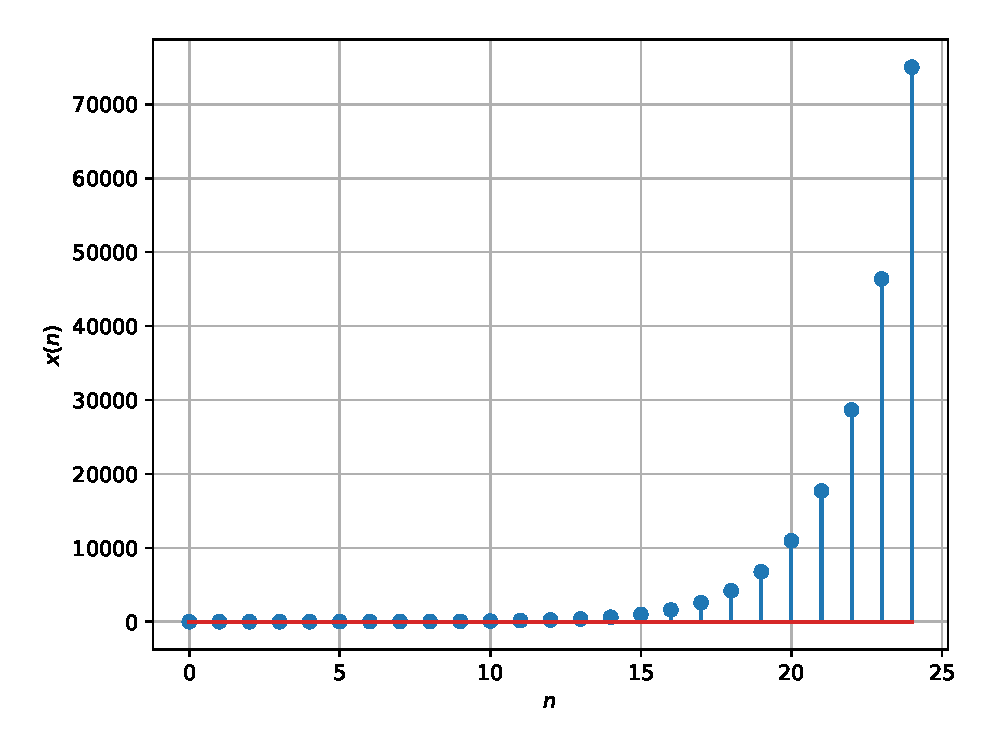
\includegraphics[width=\columnwidth]{figs/2.1}
   \caption{Plot of $x(n)$}
 \label{fig:xn}
\end{figure}
\item Find $X^{+}(z)$.

\solution Taking the one-sided $Z$-transform on both sides of \eqref{eq:10-pingala},
\begin{align}
    &\mathcal{Z}^+\sbrak{x(n + 2)} = \mathcal{Z}^+\sbrak{x(n + 1)} + \mathcal{Z}^+\sbrak{x(n)} \\
    &z^2X^+(z) - z^2x(0) - zx(1) = zX^+(z) - zx(0) + zX^+(z) \\
    &\brak{z^2 - z - 1}X^+(z) = z^2 \\
    &X^+(z) = \frac{1}{1 - z^{-1} - z^{-2}} \\
    &= \frac{1}{\brak{1 - \alpha z^{-1}}\brak{1 - \beta z^{-1}}}, \quad |z| > \alpha
    \label{eq:X-z}
\end{align}
\item Find $x(n)$.

\solution Expanding $X^+(z)$ in \eqref{eq:X-z} using partial fractions, we get
\begin{align}
    X^+(z) &= \frac{1}{\brak{\alpha - \beta}z^{-1}}\sbrak{\frac{1}{1 - \alpha z^{-1}} - \frac{1}{1 - \beta z^{-1}}} \\
           &= \frac{1}{\brak{\alpha - \beta}}\sum_{n = 0}^{\infty}\brak{\alpha^n - \beta^n}z^{-n + 1} \\
           &= \sum_{n = 1}^{\infty}\frac{\alpha^{n} - \beta^{n}}{\alpha - \beta}z^{-n + 1} \\
           &= \sum_{k = 0}^{\infty}\frac{\alpha^{k + 1} - \beta^{k + 1}}{\alpha - \beta}z^{-k}
\end{align}
where $k := n + 1$. Thus,
\begin{align}
    x(n) = \frac{\alpha^{n + 1} - \beta^{n + 1}}{\alpha - \beta}u(n) = a_{n + 1}u(n)
    \label{eq:x-n-def}
\end{align}
	\item Sketch 
\begin{align}
	y(n) = x\brak{n-1} + x\brak{n+1},  \quad n \ge 0
	\label{eq:10-orig-diff-rev}
\end{align}

\solution
\begin{lstlisting}
https://raw.githubusercontent.com/LokeshBadisa/EE3900-Linear-Systems-and-Signal-Processing/main/pingala/codes/2.2.py
\end{lstlisting}

\begin{figure}[!ht]
    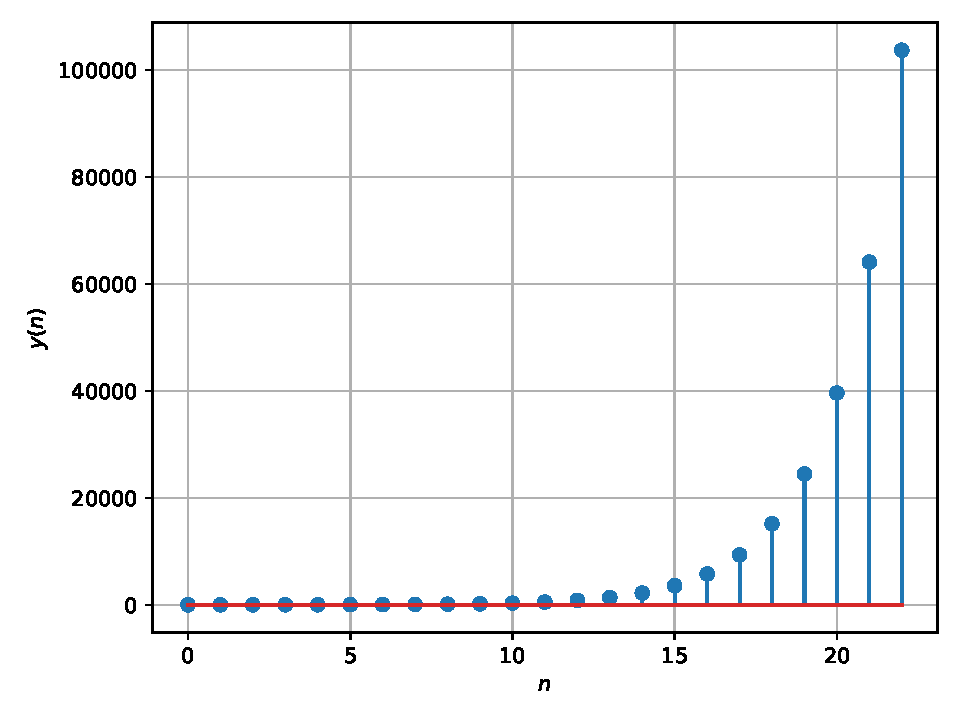
\includegraphics[width=\columnwidth]{figs/2.2}
   \caption{Plot of $y(n)$}
  \label{fig:yn}
\end{figure}
\item Find $Y^{+}(z)$. 

\solution Taking the one-sided $Z$-transform on both sides of \eqref{eq:10-orig-diff-rev},
\begin{align}
&\mathcal{Z}^+\sbrak{y(n)} = \mathcal{Z}^+\sbrak{x(n + 1)} + \mathcal{Z}^+\sbrak{x(n - 1)} \\
&Y^+(z) = zX^+(z) - zx(0) + z^{-1}X^+(z) + zx(-1) \\
&= \frac{z + z^{-1}}{1 - z^{-1} - z^{-2}} - z \\
&= \frac{1 + 2z^{-1}}{1 - z^{-1} - z^{-2}}, \quad |z| > \alpha
\end{align}
since $x(n) = 0\ \forall\ n < 0$.
\item Find $y(n)$.
    \label{pr:1-3}

\solution Using \eqref{eq:X-z},
\begin{align}
    Y^+(z) &= (1 + 2z^{-1})\sum_{n = 0}^{\infty}x(n)z^{-n} \\
           &= \sum_{n = 0}^{\infty}x(n)z^{-n} + \sum_{n = 1}^{\infty}2x(n - 1)z^{-n} \\
           &= x(0) + \sum_{n = 1}^{\infty}\brak{x(n) + 2x(n - 1)}z^{-n}
\end{align}
Thus, $y(0) = x(0) = 1$ and for $n \ge 1$, using the fact that $\alpha$ and 
$\beta$ are the roots of the equation $z^2 - z - 1 = 0$,
\begin{align}
    y(n) &= \frac{\brak{\alpha^{n + 1} - \beta^{n + 1}} + \brak{2\alpha^n + 2\beta^n}}{\alpha - \beta} \\
         &= \frac{\brak{\alpha^{n + 2} - \beta^{n + 2}} + \brak{\alpha^{n} + \beta^{n}}}{\alpha - \beta} \label{eq:y-b} \\
         &= \frac{\brak{\alpha^{n + 2} - \beta^{n + 2}} - \alpha\beta\brak{\alpha^{n} + \beta^{n}}}{\alpha - \beta} \\
         &= \frac{\brak{\alpha - \beta}\brak{\alpha^{n + 1} + \beta^{n + 1}}}{\alpha - \beta} \\
         &= \alpha^{n + 1} + \beta^{n + 1}
\end{align}
Thus, $y(n) = \alpha^{n + 1} + \beta^{n + 1}$ for $n \geq 0$ as $\alpha + \beta = 1$.
Comparing \eqref{eq:y-b} with the definition of $b_n$, we see that $y(n) = b_{n + 1}$.
Hence, $b_n = \alpha^n + \beta^n$.
\end{enumerate}
\section{Power of the Z transform}
\begin{enumerate}[label=\thesection.\arabic*,ref=\thesection.\theenumi]
\item Show that 
\begin{align}
	\sum_{k=1}^{n}a_k = 
	\sum_{k=0}^{n-1}x(k) = x(n)*u(n-1)
\end{align}

\solution From \eqref{eq:x-n-def}, and noting that $x(n) = 0\ \forall\ n < 0$,
\begin{align}
    \sum_{k=1}^{n}a_k &= \sum_{k=0}^{n-1}x(k) \\
                      &= \sum_{k = -\infty}^{n - 1}x(k) \\
                      &= \sum_{k = -\infty}^{\infty}x(k)u(n - 1 - k) \\
                      &= x(n)*u(n - 1)
\end{align}
\item Show that 
\begin{align}
a_{n+2}-1, \quad n \ge 1
\end{align}
can be expressed as 
\begin{align}
	\sbrak{x\brak{n+1}-1}u\brak{n}
\end{align}

\solution From \eqref{eq:x-n-def},
\begin{align}
    a_{n+2} - 1 = \sbrak{x(n + 1) - 1}, \quad n \ge 0
\end{align}
and so, using the definition of $u(n)$,
\begin{align}
    a_{n+2} - 1 = \sbrak{x(n + 1) - 1}u(n)
\end{align}

\item Show that 
\begin{align}
	\sum_{k=1}^{\infty}\frac{a_k}{10^k}= 
	\frac{1}{10}\sum_{k=0}^{\infty}\frac{x\brak{k}}{10^k} =\frac{1}{10}X^{+}\brak{{10}}
\end{align}
\label{pr:1-2}
\solution 
\begin{align}
    \sum_{k=1}^{\infty}\frac{a_k}{10^k} &= \frac{1}{10}\sum_{k = 0}^{\infty}\frac{a_{k+1}}{10^k} \\
                                        &= \frac{1}{10}\sum_{k = 0}^{\infty}\frac{x(k)}{10^k} \\
                                        &= \frac{1}{10}X^+(z) \\
                                        &= \frac{1}{10}\times\frac{100}{89} = \frac{10}{89}
\end{align}
\item Show that 
\begin{align}
	\alpha^n + \beta^n, \quad n \ge 1
    \label{eq:yn-exp}
\end{align}
can be expressed as 
\begin{align}
	w(n) = \brak{\alpha^{n+1} + \beta^{n+1}}u(n)
\end{align}
and find $W(z)$.

\solution Putting $n = k + 1$ in \eqref{eq:yn-exp} and using the definition of $u(n)$, 
\begin{align}
\alpha^n + \beta^n = \brak{\alpha^{k + 1} + \beta^{k + 1}}u(k)
\end{align}
Hence, \eqref{eq:yn-exp} can be expressed as
\begin{align}
w(n) = \brak{\alpha^{n+1} + \beta^{n+1}}u(n) = y(n)
\end{align}
Therefore,
\begin{align}
    W(z) = Y(z) = \frac{1 + 2z^{-1}}{1 - z^{-1} - z^{-2}}
\end{align}
 \item Show that 
\begin{align}
	\sum_{k=1}^{\infty}\frac{b_k}{10^k} =
	\frac{1}{10}\sum_{k=0}^{\infty}\frac{y\brak{k}}{10^k} =\frac{1}{10}Y^{+}\brak{{10}}
\end{align}
\label{pr:1-4}
\solution
\begin{align}
    \sum_{k=1}^{\infty}\frac{b_k}{10^k} &= \frac{1}{10}\sum_{k = 0}^{\infty}\frac{b_{k+1}}{10^k} \\
                                        &= \frac{1}{10}\sum_{k = 0}^{\infty}\frac{y(k)}{10^k} \\
                                        &= \frac{1}{10}Y^+(z) \\
                                        &= \frac{1}{10}\times\frac{120}{89} = \frac{12}{89}
\end{align}
\item Solve the JEE 2019 problem.

\solution We know that
\begin{align}
    \sum_{k = 1}^{n}a_k = x(n)*u(n - 1)
\end{align}
But
\begin{align}
    &x(n)*u(n - 1) \ztrans X(z)z^{-1}U(z) \\
    &= \frac{z^{-1}}{\brak{1 - z^{-1} - z^{-2}}\brak{1 - z^{-1}}} \\
    &= z\sbrak{\frac{1}{1 - z^{-1} - z^{-2}} - \frac{1}{1 - z^{-1}}} \\
    &\ztrans z\sum_{n = 0}^{\infty}\brak{x(n) - 1}z^{-n} \\
    &= \sum_{n = 0}^{\infty}\brak{x(n) - 1}z^{-n + 1} \\
    &= \sum_{n = 0}^{\infty}\brak{x(n + 1) - 1}z^{-n} \\
\end{align}
From \eqref{eq:x-n-def}, we get
\begin{align}
    \sum_{k = 1}^{n}a_k = a_{n+2} - 1
\end{align}
We have already established the remaining options in order in the problems
\eqref{pr:1-2}, \eqref{pr:1-3}, \eqref{pr:1-4}. Therefore, options 1, 2,
and 3 are correct and option 4 is incorrect.
\end{enumerate}
\end{document}